% 2019 上海春季卷第 17 题；透视投影为示意，M、N 按两条线段中点构造。
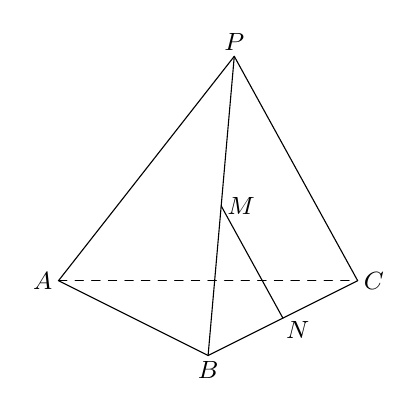
\begin{tikzpicture}[scale=0.95,line cap=round,line join=round,font=\small]
  \coordinate (A) at (0,1);
  \coordinate (B) at (2,0);
  \coordinate (C) at (4,1);
  \coordinate (P) at (2.35,4);
  \coordinate (M) at (2.175,2);
  \coordinate (N) at (3,0.5);

  \draw[dashed] (A) -- (C);
  \draw (P) -- (A) -- (B) -- (C) -- cycle;
  \draw (P) -- (B);
  \draw (M) -- (N);

  \node[left,inner sep=2pt] at (A) {$A$};
  \node[below,inner sep=2pt] at (B) {$B$};
  \node[right,inner sep=2pt] at (C) {$C$};
  \node[above,inner sep=2pt] at (P) {$P$};
  \node[right,inner sep=2pt] at (M) {$M$};
  \node[below right,inner sep=1pt] at (N) {$N$};
\end{tikzpicture}
